\documentclass[12pt,a4paper]{article}

\usepackage{lmodern}
\usepackage[T1]{fontenc}
\usepackage[utf8]{inputenc}
\usepackage[italian]{babel}

\usepackage{hyperref}
\usepackage{graphicx}
\graphicspath{{img/}}
\usepackage{float}

\usepackage{titlesec}

\setcounter{secnumdepth}{4}

\titleformat{\paragraph}
{\normalfont\normalsize\bfseries}{\theparagraph}{1em}{}
\titlespacing*{\paragraph}
{0pt}{3.25ex plus 1ex minus .2ex}{1.5ex plus .2ex}

\begin{document}
\begin{titlepage}
	\centering
	\vspace*{4.5cm}
	{\scshape\LARGE \textbf{EmpireCon} \par}
	\vspace{0.5cm}
	{\Large \textbf{\textit{Relazione sul progetto per il corso di Tecnologie Web}}\par}
	\vspace{1cm}
	{\Large Andrea Cardin, 1030310\par}
	{\Large Andrea Nalesso, 1026100\par}
	{\Large Ismaele Gobbo, 1028902\par}
	\vspace*{\fill}
\end{titlepage}

\tableofcontents
\newpage

% Come inserire una sezione
% \section{Nome sezione}
% \input{sections/nome file latex della sezione senza .tex}
% \newpage
% Esempio:
% \section{Introduzione}
% placeholder
% \newpage

\section{Introduzione}
placeholder

\section{Progettazione}
\subsection{Struttura del sito}
Ogni pagina del sito è formata dai seguenti elementi:
\begin{itemize}
	\item Header;
	\item breadcrumb;
	\item box che permette il login o mostra l'account con cui si è autenticati;
	\item menù;
	\item contenuto della pagina;
	\item footer.
\end{itemize}

\subsubsection{Mappa del sito}
\begin{figure}[H]
	\centering
	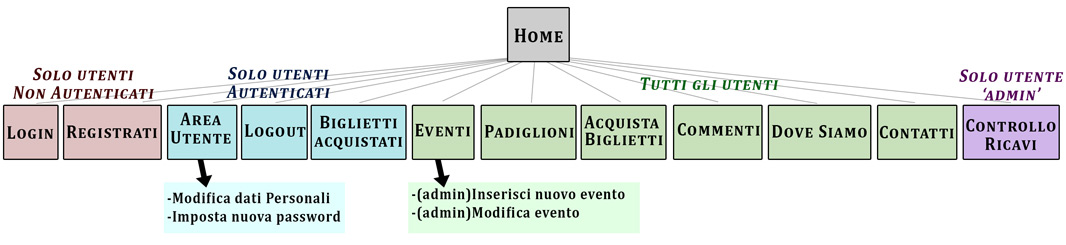
\includegraphics[width=16cm]{mappa-sito-small}
	\caption{Mappa del sito.}
\end{figure}
Oltre alla home page, che è concettualmente la radice del sito ed è ovviamente accessibile a tutti gli utenti, le varie pagine sono concettualmente suddivise nelle seguenti aree basate sull'attore che le andrà ad utilizzare:
\begin{itemize}
	\item Per soli utenti non autenticati;
	\item per soli utenti autenticati;
	\item per tutti gli utenti;
	\item per il solo utente amministratore.
\end{itemize}

\paragraph{Home page}
È, concettualmente, la radice del sito, nonché la pagina in cui l'utente si dovrebbe ritrovare quando si collega al sito. Contiene un paragrafo introduttivo di benvenuto e presentazione, seguito dalle news riguardante l'evento.

\paragraph{Per soli utenti non autenticati}
Quest'area contiene le pagine destinate agli utenti non autenticati, permettendo loro di interagire con le funzioni di autenticazione e registrazione al sito.
Pagine che ne fanno parte:
\begin{itemize}
	\item Login;
	\item Registrazione.
\end{itemize}

\paragraph{Per soli utenti autenticati}
Quest'area contiene le pagine che possono essere visitate o accedute solo dagli utenti che hanno eseguito l'autenticazione al sito. Le pagine di questa area permettono di interagire con gli aspetti relativi alla gestione del proprio account, come ad esempio la modifica dei dati personali o della password, la possibilità di effettuare il logout e, infine, un elenco dei biglietti acquistati da quell'account. L'accesso ad una di queste pagine da parte di un utente non autenticato produce un errore oppure, nel caso di area utente e logout, un reindirizzamento. Inoltre, ad un utente non autenticato non sono mai mostrati collegamenti a queste pagine.
Pagine che ne fanno parte:
\begin{itemize}
	\item Area Utente;
	\item Logout;
	\item Biglietti Acquistati.
\end{itemize}

\paragraph{Per tutti gli utenti}
Queste pagine sono accessibili a tutti gli utenti, a prescindere dal loro stato di autenticazione, tramite il menù.
Contengono i contenuti veri e propri del sito, con informazioni sulla fiera, l'acquisto dei biglietti e la possibilità di lasciare dei commenti.
Pagine che ne fanno parte:
\begin{itemize}
	\item Eventi:
		Presenta la lista di tutti gli eventi che si terranno nel corso della fiera. Per ogni evento vengono offerte informazioni utili quali la data, l'ora di inizio, l'ora di fine, il padiglione in cui si svolgeranno ed una descrizione.
		L'utente amministratore ha la possibilità di svolgere alcune funzioni aggiuntive: l'inserimento di un nuovo evento e la modifica o cancellazione di un evento già inserito.
	\item Padiglioni:
		Mostra l'elenco dei padiglioni presenti nella fiera suddivisi per settori. Inoltre mostra anche una mappa con la posizione di ogni padiglione. Il contenuto è uguale per tutte le categorie di utenti.
	\item Acquista biglietti:
		Elenca a tutti i tipi di utenti le varie tipologie di biglietti disponibili ed il loro prezzo. Ad un utente autenticato offre anche la possibilità di procedere all'acquisto di uno o più biglietti.
	\item Commenti:
		Rappresenta il "libro ospiti" del sito. Gli utenti di tutte le categorie possono leggere i commenti. Un utente autenticato ha a disposizione la funzione di eliminazione per i commenti da lui inviati, mentre l'utente amministratore può eliminare qualsiasi commento.
	\item Dove siamo:
		Offre indicazioni per raggiungere il luogo della fiera. Il contenuto è uguale per tutte le categorie di utenti.
	\item Contatti:
		Contiene informazioni su come contattare gli organizzatori della fiera. Il contenuto è uguale per tutte le categorie di utenti.
\end{itemize}

\paragraph{Per il solo utente amministratore}
A questa categoria appartiene una sola pagina: Controllo ricavi.
Questa pagina è destinata all'utente amministratore e presenta in forma tabellare il resoconto sui biglietti venduti e sui guadagni.

\subsection{Layout}
\textbf{TODO}

\subsection{scelte progettuali}
\textbf{TODO}

	

\section{Realizzazione}
\subsection{Perl}
Per la componente dinamica e di back-end del sito è stato utilizzato il linguaggio Perl come richiesto dalle specifiche del progetto. La versione utilizzata è quella installata nel server tecweb dell'Università. \newline
Le librerie principali utilizzate, dopo una iniziale valutazione tra quelle disponibili, sono state:
\begin{itemize}
	\item \textbf{CGI:} Per la gestione delle connessioni, il passaggio dei parametri HTTP tra le pagine e la gestione delle sessioni;
	\item \textbf{LibXML:} Per la gestione e manipolazione dei file XML;
	\item \textbf{HTML::Template:} Per la costruzione e presentazione dei contenuti. 
\end{itemize}
Tutte le pagine del sito sono dinamiche e realizzate in Perl per poter gestire le sessioni e le operazioni degli utenti.
Ogni pagina è realizzata in maniera modulare tramite template innestati. L'elemento principale è il template \textit{Page} che contiene il menù e il breadcrumb del sito, nonché richiama l'inclusione di altri template: \textit{Header}, che contiene il blocco \textit{head} della pagina, ed il \textit{Footer}. Oltre ai template sopraccitati, che sono presenti in ogni pagina e adattati tramite variabili dinamiche, il template Page richiede l'inclusione del contenuto vero e proprio della pagina, che è stato realizzato sotto forma di un template specifico per ogni pagina del sito. La dinamicità dei contenuti è ottenuta tramite l'interazione (sotto forma di variabili) tra il template del contenuto e la corrispondente pagina cgi.
La libreria LibXML è stata scelta perché è risultata essere la più completa e di più semplice utilizzo.

\subsection{XML}
Il progetto include quattro file XML utilizzati per salvare in modo persistente i dati. Per ogni file XML è stato realizzato un XMLSchema che ne definisce la struttura. Gli schemi sono stati realizzati utilizzando il modello \textit{Tende alla Veneziana}. Utilizzando il tool \textit{xmllint} gli schemi sono stati validati contro lo schema che definisce gli XMLSchema fornito dal W3C, mentre i file XML sono stati validati contro i rispettivi schemi da noi scritti. \newline
I file XML realizzati sono:
\begin{itemize}
	\item \textbf{utenti:} contiene tutti i dati degli utenti che si registrano al sito, compresi username e password necessari per l'autenticazione. La password viene cifrata con una funzione di hash prima di essere salvata;
	\item \textbf{commenti:} contiene tutti i commenti inviati dagli utenti;
	\item \textbf{eventi:} contiene tutti gli eventi che avranno luogo durante la fiera;
	\item \textbf{biglietti:} contiene la lista di tutti i biglietti acquistati.
\end{itemize}

\end{document}
